\chapter{Introduction}

Scientists, engineers, and researchers use wireless sensor networks (WSN) for a
wide array of applications. Many of these applications rely on knowledge on the
precise position of each node in the networks


\section{Motivation} For the first round of testing, chosen more as an excercise
in the simulation analysis package in MATLAB\copyright, 4 anchor nodes are
placed at the closest node the the 45-degree axes, with increasing distance from
the center. shows the positions for each iteration.

%\begin{figure} % % Requires \usepackage{graphicx} % \centering %
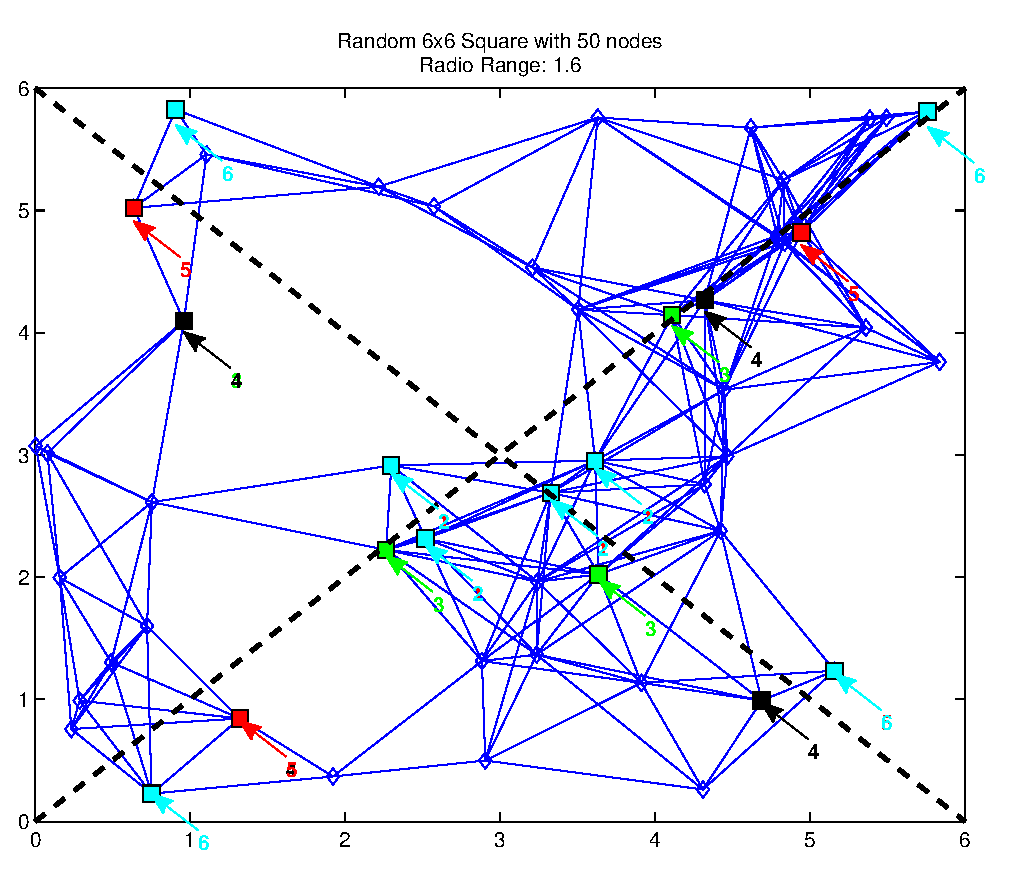
\includegraphics[width=4in]{../cca/results/45DegreeAxis_Random/networkRandom6x6Squarewith50nodes1-6Radius.eps}\\
% \caption{The random network used, showing the 6 position sets of anchors.} %
\label{fig:45DegreeAxisRandomNetwork} %\end{figure}

%\begin{equation}\label{eqn:newton_law} %    F = Ma %\end{equation}
%Paragraph referencing an equation \ref{eqn:newton_law}.
